\chapter{Deep Neural Networks}
\label{chap:DeepNeuralNetwork}

This chapter talks mainly about the~model we decided to use. First, we describe the~full pipeline of a~traditional OMR system. Many of these steps are shared between traditional and deep learning approaches. Then we will talk about the~deep learning approaches that can be taken. Neural networks can replace parts of a~traditional pipeline, or they can be used in an~end-to-end setting, where the~neural network replaces the~most difficult core of the~pipeline. We will describe our architecture consisting of a~convolutional block, recurrent block, and the~connectionist temporal classification (CTC) loss function. The~following sections describe in more detail what a~neural network is and how the~individual blocks of our model work internally. The~last section explains how CTC works and what are its pros and cons, compared to the~approach described in the~HMR baseline article (\cite{HmrBaseline}).


\section{Traditional Approaches}

A~musical score intended for OMR typically begins as a~raster image. This image is a~photo or a~scan of a~real-world sheet of paper. The~image needs to be prepared first. We need to find the~sheet of paper in the~image and correct any rotation or~perspective distortion. Scanned images are easier to~prepare because they do not contain any perspective deformation and lighting artifacts. Searching for the~paper in the~image can be performed using many approaches, e.g. by using maximally stable extremal regions (\cite{MSER}). We can detect staff lines using Hough transform (\cite{Hough}). We can then use this information to remove any affine distortion of the~image.

The~next step is performing some color normalization and binarization. There might be a~light-intensity gradient over the~image, so we do some automatic contrasting to bring the~lightness to a~constant level across the~image. Median filtering can be applied to remove noise (\cite{MedianFiltering}). Conversion to a~grayscale image is often used since colors are not useful to OMR. The~image can then be binarized to further remove unnecessary information. Many thresholding algorithms can be used for this step, many of which are implemented in the~OpenCV\footnote{\href{https://opencv.org/}{https://opencv.org/}} library. Binarization is important for traditional approaches since they often use methods based on connected components to detect individual symbols. Neural networks could benefit from non-binarized images since binarization can create aliasing artifacts that distort the~input image on the~pixel level.

The~steps described above are shared by both traditional and neural network-based approaches. Traditional approaches now usually perform staff line removal. This step lets methods based on~connected components to become useful. Staff localization may be an~important part of this step. Symbols then need to be segmented and classified separately. Meaning is then reconstructed by looking at the~relationships between all the~classified symbols. With the~musical score understood at the~symbol level, the~extracted information can be converted to some final representation (MusicXML, MEI, MIDI).


\section{Deep Learning Approaches}

Deep learning is a~class of machine learning that focuses on deep neural networks. Deep learning has risen over the~past two decades and became a~very powerful tool for solving many problems, especially classification problems regarding computer vision. Neural networks can be used in many places throughout the~pipeline of a~traditional OMR system. They can be used for staff line removal (\cite{CalvoZaragoza2017}), symbol classification (\cite{Lee2016}), or even symbol detection (\cite{Pacha2018}).

Recently, neural networks have been used to tackle the~problem of~OMR in an~end-to-end fashion (\cite{Primus}, \cite{HmrBaseline}). This approach allows us to replace many stages of the~pipeline with a~single model. The input sheet of music is usually processed staff by staff, so an~initial segmentation of staves is required. This step is, however, very robust and can be performed reliably.

The~main steps unified by an~end-to-end system are segmentation, symbol classification, and part of the~relationship extraction. This means we do not need to explicitly specify the~structure of this part of the~pipeline, which saves a~lot of time and thinking. Also, any intermediate features that would be extracted (like noteheads) need not be specified. The deep neural network can learn, what those features are. Moreover, it can adapt these features to the problem better than a~human could.

Deep learning, especially in an~end-to-end approach also has some drawbacks. The first is bound to the ability of the~model to learn the~solution from data. While it is very helpful, that we do not have to design part of our OMR system manually, it is often very difficult to acquire enough high-quality data for the~training. Also, the~more complex our model is and the~more learned parameters it has, the~more training data it requires. The~data also needs to be of high quality. Ambiguity and mistakes in annotations lead to poor performance of the~resulting model. The~trained model can only ever be as good as its training data.

The second drawback is the~very difficult nature of debugging the~model. A neural network is by design a~black box and we cannot easily assign specific meaning to any of its internal parts. The process of fixing a~mistake the model makes is tedious and requires a~lot of experimentation and re-training.


\section{Our Architecture}

As stated in the~title of this thesis, we decided to explore the~end-to-end approach to OMR using deep neural networks. We were primarily inspired by these three models:

\begin{itemize}
\item End-to-End Neural Optical Music Recognition of Monophonic Scores by Calvo-Zaragoza and Rizo (\cite{Primus})
\item SimpleHTR by Harald Scheidl\footnote{\href{https://github.com/githubharald/SimpleHTR}{https://github.com/githubharald/SimpleHTR}}
\item From Optical Music Recognition to Handwritten Music Recognition: A baseline (\cite{HmrBaseline})
\end{itemize}

All of these models share the~same high-level structure. They combine a~convolutional neural network (CNN) with a~recurrent neural network (RNN). This combination is sometimes called RCNN architecture. Convolutional neural networks are used in image processing. Their architecture is inspired by the~way filters work in computer graphics (convolving a~kernel over the~source image). They learn to extract edges, corners, and then even more abstract features like noteheads and stems. Recurrent neural networks are used for sequence processing (text and speech). They have been designed to carry state information throughout the~input sequence. In our case, they learn to propagate information horizontally --- like inferring pitch of an~accidental from the~pitch of a~neighboring note. The CNN block learns to extract features that the RNN block then learns to combine into more abstract features.

\begin{figure}[h]
    \centering
    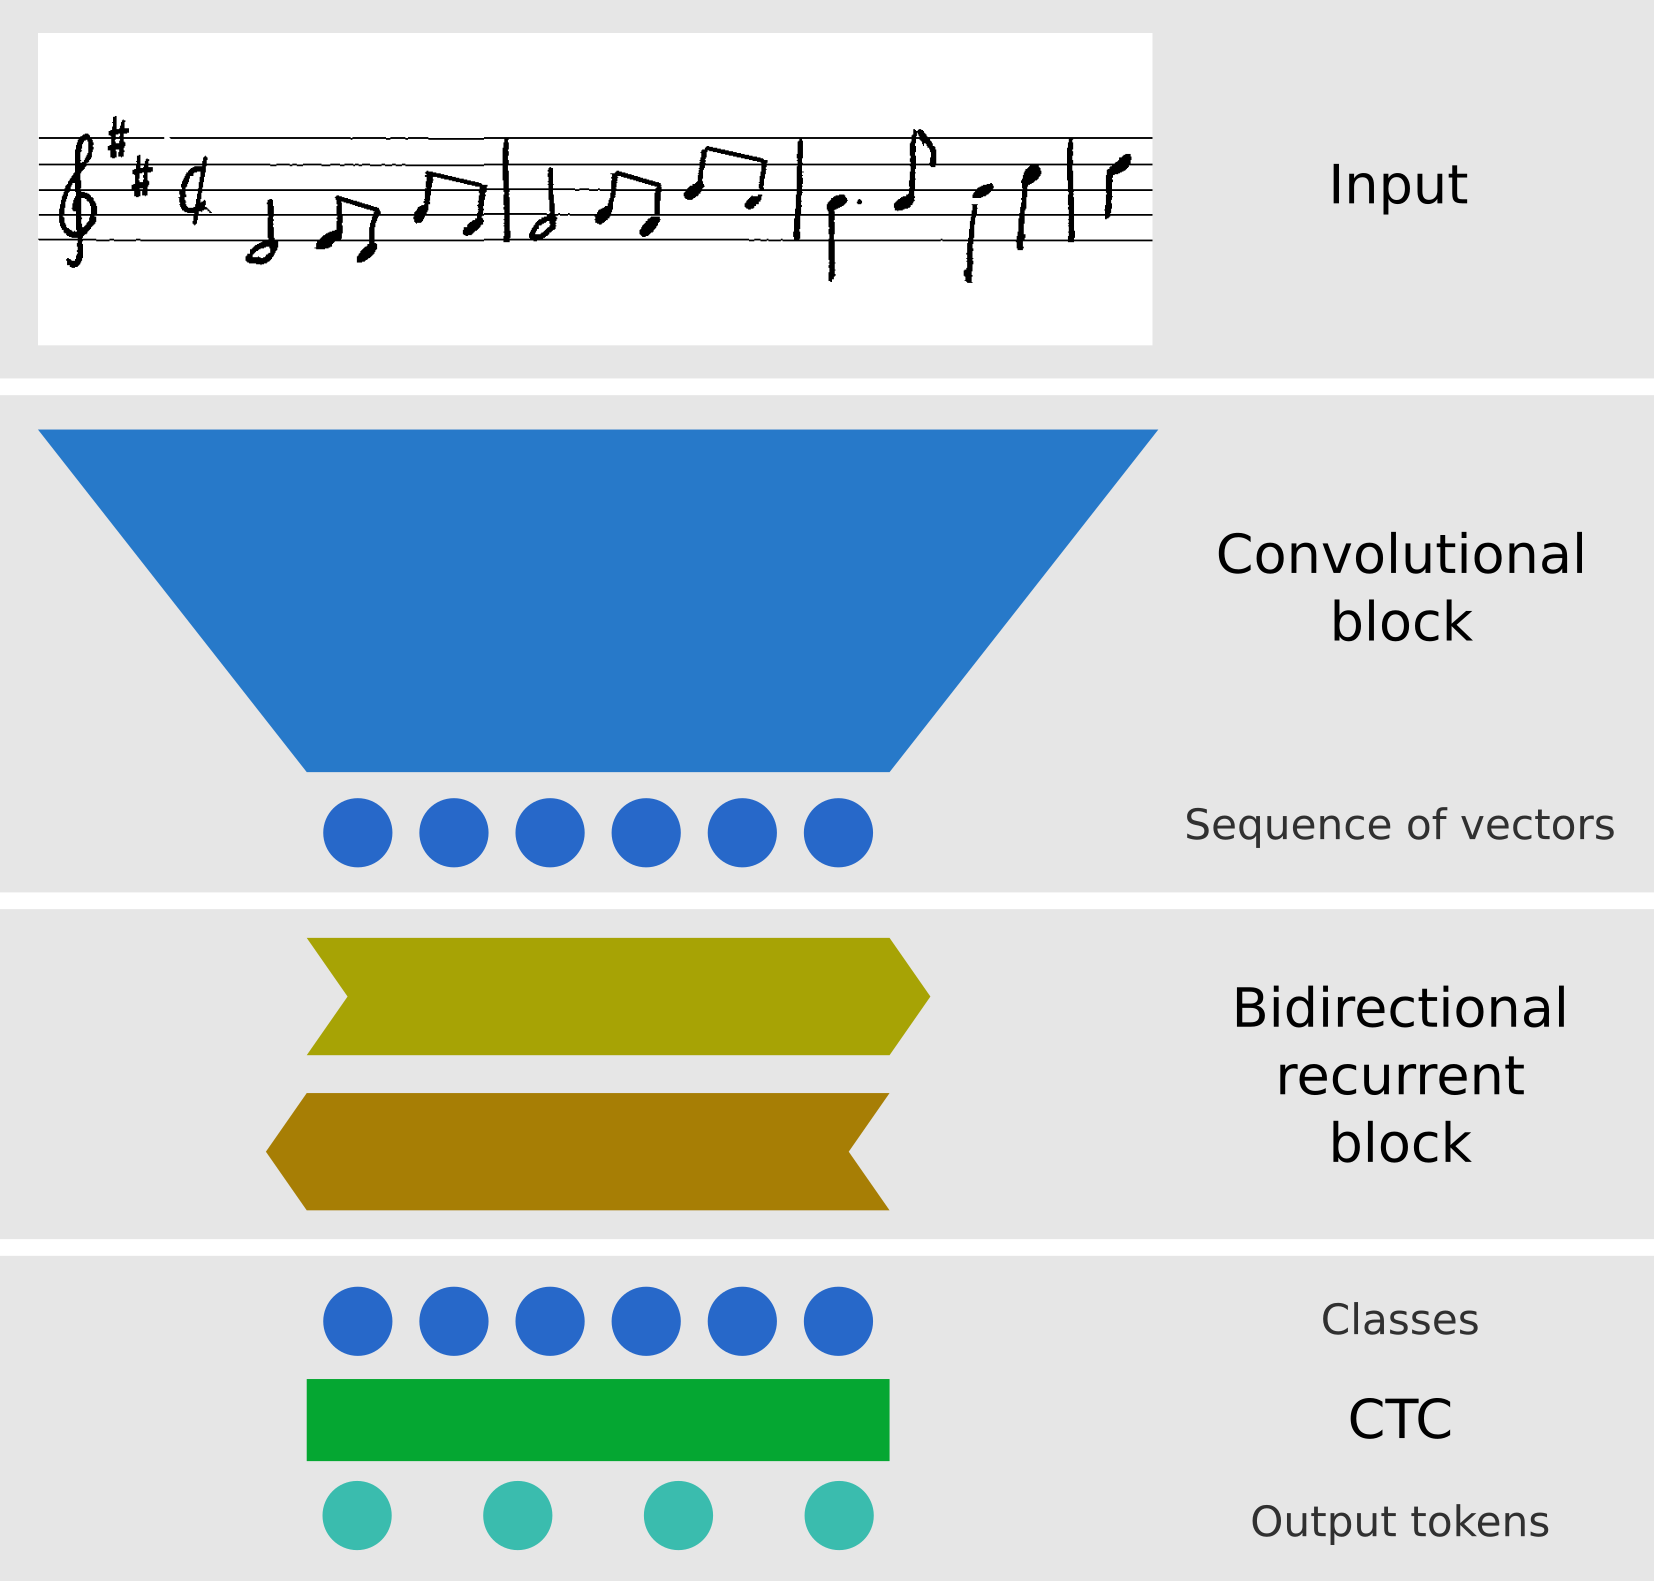
\includegraphics[width=140mm]{../img/network-architecture}
    \caption{Diagram of our model --- a RCNN network with CTC loss function. Detailed list of layers with all parameters can be found in table~\ref{tab6:NetworkLayers}}
    \label{fig3:NetworkArchitecture}
\end{figure}

The~RNN block can be followed by fully connected layers that further refine the~result, although these layers are not necessary and our architecture does not contain them. This may be due to the fact that our encoding is very close to the~symbolic visual representation and~so most of the~heavy lifting is probably performed in the~CNN block.

The~final layer outputs a~sequence of vectors, where each vector represents one time-step (horizontal slice of the~input image). Values in such vector correspond to probabilities of individual output classes (tokens) at that given time-step. One additional class \emph{blank} is added, which represents "no symbol present". The~most likely class for each time-step is selected and then repetitions of the~same class are collapsed into one token. Lastly, all the~blank symbols are removed. The~remaining sequence of classes is mapped directly onto annotation tokens of the~Mashcima encoding explained in the~chapter \ref{chap:MusicRepresentation}. This approach is called greedy CTC decoding (\cite{CTC}) and is used during training. For evaluation, a more advanced method is used, called beam search decoding (\cite{CtcBeamSearch}).

When training, the~loss is computed using the~connectionist temporal classification. The~loss function provides a~gradient for improving the~network. This gradient is then calculated for the~entire network using the~backpropagation algorithm (\cite{Goodfellow-et-al-2016}). Parameters are then updated using the~adaptive learning rate optimizer (Adam) (\cite{AdamOptimizer}).

The~values of all hyperparameters, including sizes and types of all layers, are specified in the~section \ref{sec:ArchitectureTrainingEvaluation}.


\section{Neural Network}

A~neural network is a~model inspired by the~human brain. Its~core building block is a~perceptron (analogous to a~neuron in the~brain). Perceptron is a~node that has several inputs (real numbers), combines them, and produces a~single output value. The mathematical description is the following:

$$
    y = \varphi(w \cdot x + b)
$$

Vector $x$ contains all the~input values. It is multiplied by a~vector of weights $w$ and a~constant scalar bias $b$ is added. The~result is passed through an~activation function $\varphi$ that produces the~output value $y$. The~core idea behind this model is that a~perceptron activates (fires) when enough inputs activate. Weights and the~bias are parameters that allow the~perceptron to learn - to detect a~specific pattern in the~input values. The~activation function attempts to model the~activation threshold and introduces non-linearity into the~system.

One of the~first activation functions to be used was the~sigmoid function, but~it suffered from the~problem of vanishing and exploding gradients (\cite{VanishingGradient}). The hyperbolic tangent function was then used to remedy this problem. Nowadays, rectifier function is often used ($\max(0, x)$), because it is easy to compute. Perceptrons with this function are called rectified linear units (ReLU). It~also has some problems, so~leaky ReLU can be used to address them (\cite{Maas2013RectifierNI}).

\begin{figure}[h]
    \centering
    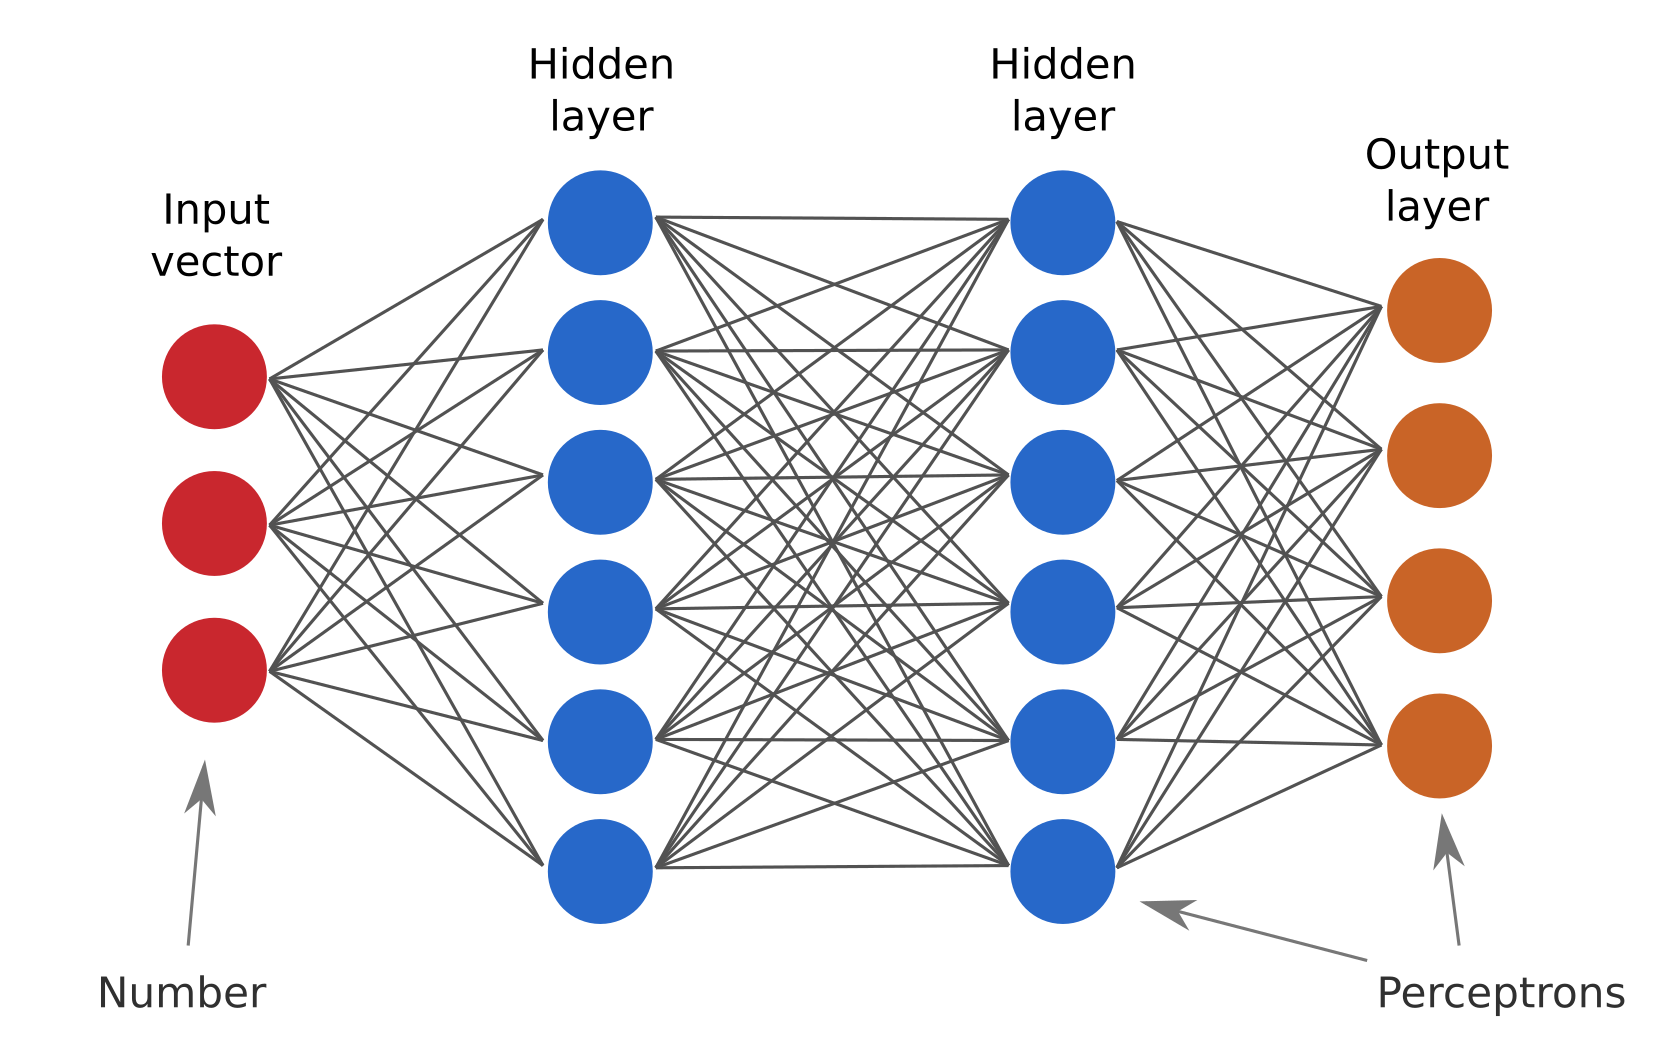
\includegraphics[width=140mm]{../img/neural-network}
    \caption{Fully-connected neural network with 3 layers.}
    \label{fig3:NeuralNetwork}
\end{figure}

Perceptrons can be interconnected to form neural networks. A~typical architecture is a~feedforward neural network (FNN). It~organizes perceptrons into layers, through which information flows in one direction. The resulting graph is directed and acyclic, which allows us to understand the~whole network as a~complex mathematical function and lets us train it using the~backpropagation and gradient descent algorithms (\cite{Goodfellow-et-al-2016}).

The~simplest feedforward network is a~network with dense (fully connected) layers. Each perceptron in a~given layer receives input as the~output of all perceptrons in the~previous layer.


\section{Convolutional Neural Network}

A~convolutional neural network (CNN) is a~kind of feedforward network. It~is ideal for processing visual data. A~CNN is built primarily from two kinds of layers:

\paragraph{Convolutional layer} A~convolutional layer is similar to a~fully connected layer, but the~connections are only local. The~input and output is a~two-dimensional array of numbers (like one channel of an~image). Each perceptron takes input from only a~small window of neighboring perceptrons in the~input layer (\texttt{3x3}, \texttt{5x5}, \texttt{7x7}). Weights are represented by a~kernel of the~same size as this neighborhood window. This kernel is shared by all the~perceptrons, reducing the~number of learned arguments substantially and allowing the~layer to process images of variable sizes. There may be multiple input and output arrays (channels). In such a~case, the~convolutional layer has one kernel for each pair of channels. This architecture is inspired by the~convolution filters from computer graphics --- hence the name.

\begin{figure}[h]
    \centering
    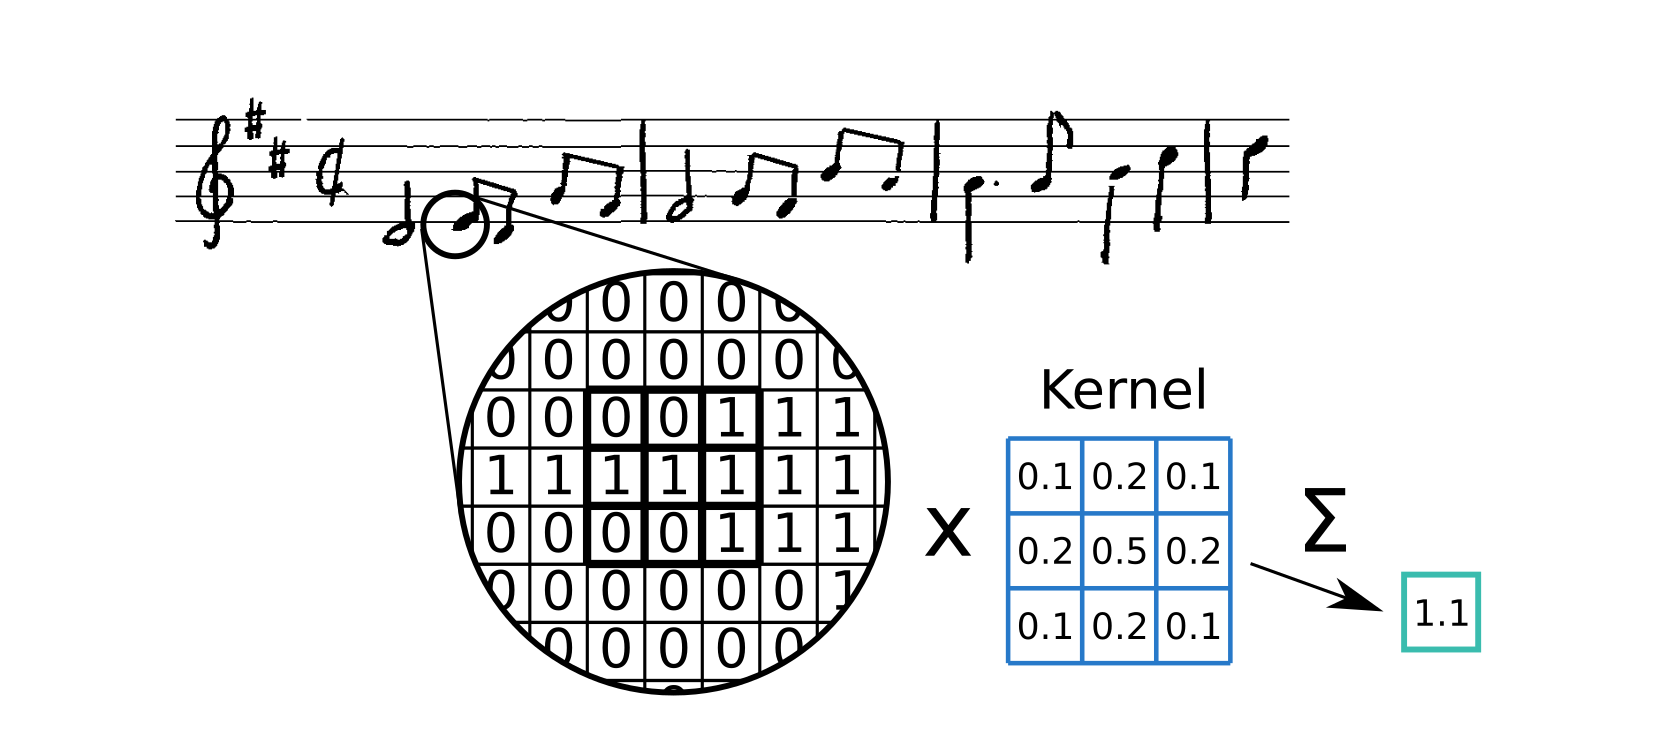
\includegraphics[width=140mm]{../img/convolution}
    \caption{Computation of one output pixel in a convolutional layer.}
    \label{fig3:Convolution}
\end{figure}

\paragraph{Pooling layer} A~pooling layer typically follows a~convolutional layer. Its~job is to downsample the~image, reducing its spatial resolution, while preserving the number of channels. The~downsampling is performed by splitting the~input into a~set of rectangular regions (that may overlap) and then reducing each region using max, sum, or average operator. Widely used is the~maximum operator and the~resulting layer is called a~\emph{max pooling layer}. The pool size is typically \texttt{2x2}.

\paragraph{Fully-connected layer} One or more fully connected layers can be added at the~end of a~CNN, to further refine features extracted by the~previous layers. This layer is often present in models performing classification because we want to reduce the~number of outputs to the~number of classes we are predicting.

A~CNN has typically many convolutional layers, combined with pooling layers. Each time the~spatial dimensions shrink in a~pooling layer, more channels are added to be able to represent more features. This forces the network to create abstractions and convert the~visual data into some abstract representation vector.


\section{Recurrent Neural Network}

A~recurrent neural network (RNN) is a~network intended for sequence processing. Input for the~network is a~sequence of vectors and the~output is a~sequence of the~same length. The~recurrent network can be understood as composed of recurrent units, each with two inputs and two outputs. A~unit accepts one vector from the~input sequence and an~old state vector. It~outputs the~corresponding vector of the~output sequence and the~new state vector. These recurrent units can be unrolled along the~input sequence and each one passes the~state vector to the next one, using it to send information along the~length of the~sequence. All instances of the~recurrent unit share the~same learned parameters and so can be unrolled to any length necessary. The~sequence dimension, where unrolling happens, is called the time dimension.

\begin{figure}[h]
    \centering
    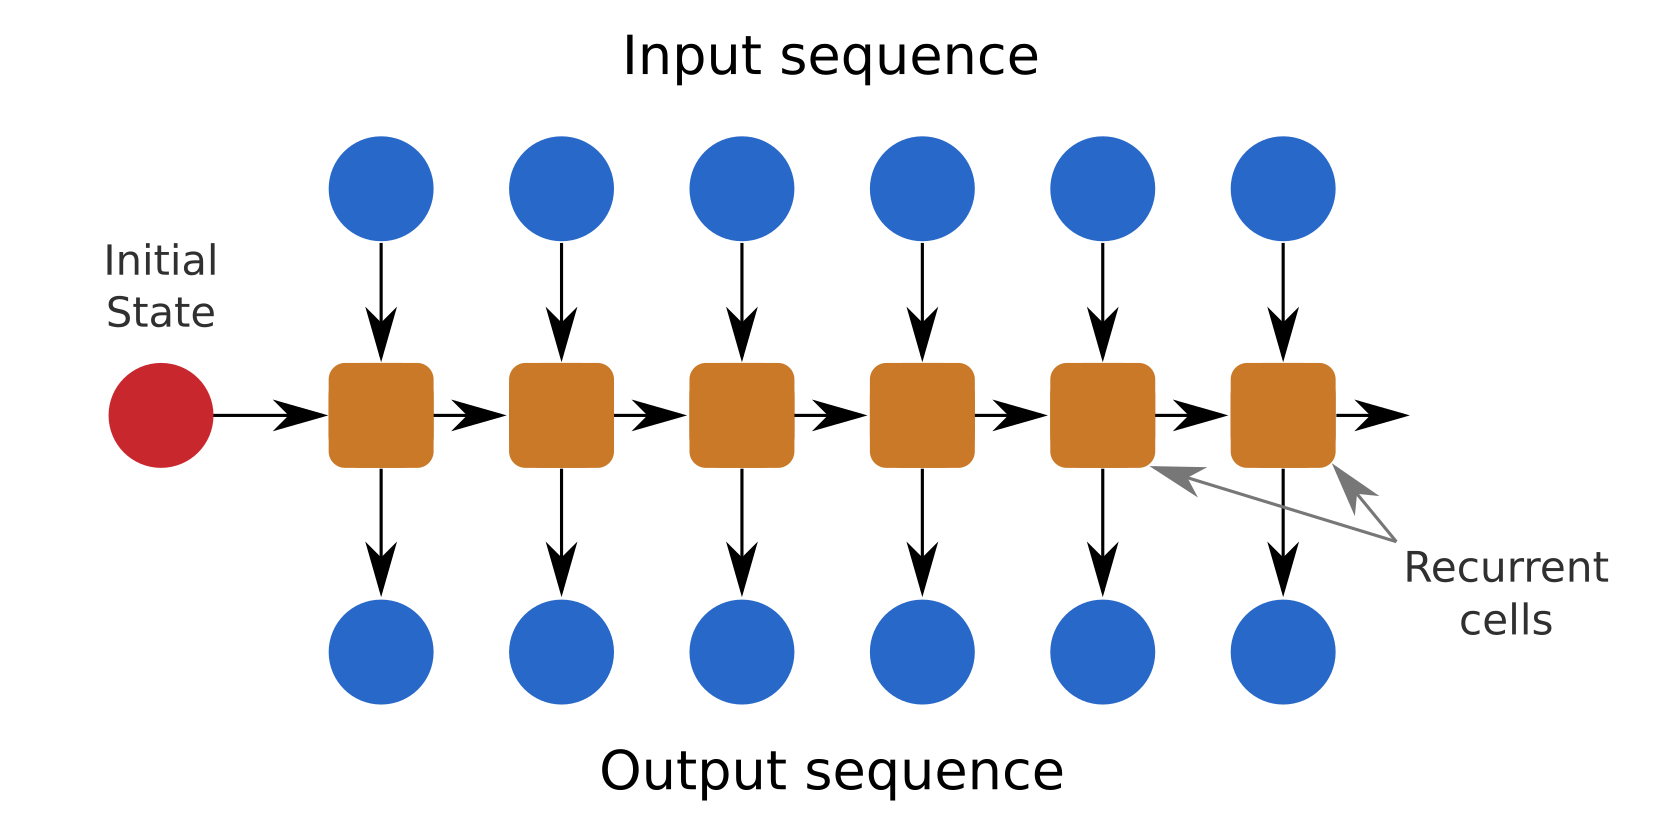
\includegraphics[width=140mm]{../img/recurrent-network}
    \caption{Unrolled recurrent units processing a sequence of vectors.}
    \label{fig3:RecurrentNetwork}
\end{figure}

The~internal architecture of a~recurrent unit may vary, but it is often a~feedforward network, where the~input and output vectors are both split into a~sequence part and a~state part. The most common recurrent unit architectures are the~long short-term memory (LSTM) (\cite{LSTM}) and the~gated recurrent unit (GRU) (\cite{GRU}). You can join two recurrent layers, passing information in opposite directions, to create a~bidirectional recurrent layer.


\section{Connectionist Temporal Classification}

A~recurrent neural network outputs a~sequence of vectors. If~these vectors are the~final output of the~model, they typically represent class probabilities for a~given time-step (we solve sequence classification). If~we did OCR, we~would have a~set of characters (an~alphabet) and the~vector would have the~same size as the~alphabet. Each value in that vector would correspond to the~probability of that given character being present at that given time-step. We could use the~softmax function (\cite{Goodfellow-et-al-2016}) to convert the perceptron activations to probabilities.

This creates a~problem when training. In~OCR, we want to produce a~sequence of letters as the~output. But one letter might span multiple time-steps in the~input. This means we not only need the~gold sequence of letters, but we also need to know at which specific time-steps the~letters are present. This mapping of output classes to specific time-steps is called \emph{alignment} and it complicates the~creation of a~training dataset.

Connectionist temporal classification (CTC) (\cite{CTC}) is an~approach that solves the~alignment issue. The CTC loss function can calculate the~loss value over all possible alignments of our gold sequence over the~output sequence. This allows us to train the~model, without having explicit alignment.

When the~model is trained, the~greedy decoding algorithm (\cite{CTC}) can be used to convert the~output vector sequence to the~proper prediction. This algorithm takes each vector of the~output sequence and selects the~most probable output class (letter). It~then collapses all repetitions of that class into one occurrence, producing the~final sequence. One special output class called \emph{blank} is introduced, to prevent two actual successive occurrences of a~given class from being collapsed into one. This symbol is, however, after collapsing removed and will never be present in the~final prediction.

There is also the~option to use the beam search decoding algorithm (\cite{CtcBeamSearch}). This algorithm keeps a~list of best decodings so~far, as the~entire decoding is being computed. Greedy decoding is a~special case of the~beam search decoding, where the~list contains only one item. All partial decodings cannot be considered, because there are exponentially many of them.

The~connectionist temporal classification has many benefits regarding the alignment problem, but it has some flaws as well. The~loss computation and the~decoding rely on the~fact, that there will be only one class predicted for each time-step. This means we cannot capture the~fact of two symbols appearing in the~input at the~same time. This happens often with music. We can solve this problem partially by utilizing the~recurrent layers. They will allow us to output simultaneous symbols sequentially, by remembering those symbols for a~while. This however increases the~length of the~final sequence, but this sequence can never be longer than the~total number of time-steps. We might run out of temporal resolution.

The~HMR baseline article (\cite{HmrBaseline}) opted not to use CTC and performed manual alignment instead. This lets them have a~model that can predict multiple symbols simultaneously. This also reduces the~complexity of the~output sequence and the~model thus need not perform much additional work as in our case (see the~section \ref{sec:Attachments} on attachment ordering).
